\chapter{Auswertung}
\label{chap:auswertung}

Die Auswertung dieser Fallstudie erfolgt mithilfe zwei verschiedener wissenschaftlicher Methoden.
Eine detaillierte Erläuterung der Methodik ist in \cref{chap:methodik} gegeben.
Zuerst werden in \cref{sec:auswertung-interviews} die durchgeführten Experteninterviews ausgewertet.
Außerdem werden in \cref{sec:auswertung-feldnotizen} die im Ver\-lauf der Anwendung des \gls{mmf} in dieser Thesis erstellten Feldnotizen ausgewertet.
Zum Abschluss dieses Kapitels werden die Ergebnisse dessen in \cref{sec:auswertung-diskussion} diskutiert und durch eine qualitative Bewertung des Refactoringprozesses durch den Autor ergänzt.

\section{Experteninterviews}
\label{sec:auswertung-interviews}

In diesem Abschnitt werden die Ergebnisse der Experteninterviews beschrieben und diskutiert.
Die Ex\-per\-ten\-inter\-views wurden mit dem Ziel durchgeführt, eine Evaluation der Anwendung des \gls{mmf}/\gls{arh} auf \jf von weiteren Personen zu erhalten, die nicht an der Durchführung beteiligt waren.
Die genaue Methodik der Interviews ist in \cref{sec:methodik-interviews} erläutert und der Leitfaden kann in \cref{chap:expert-interviews-leitfaden} gefunden werden.

Das erste Interview wurde gezielt mit dem \gls{po} von \jf durchgeführt. 
Er begleitete alle Phasen der Thesis und benötigte deshalb keine thematische Einweisung. 
der \gls{po} hat die Präambel und das Informationsmaterial erst wenige Stunden vor dem Interview erhalten.
Durch die vorherige Mitarbeit des Teilnehmers an der Thesis konnte im ersten Interview zusätzlich evaluiert werden, ob die Verständnisfragen, inhaltlichen Fragen und der Zeitrahmen passend gewählt wurden.
Den anderen Teilnehmern, die nicht mit dem Inhalt der Thesis vertraut waren, wurden vier Tage vor den Interviews eine Präambel (\cref{chap:expert-interviews-preamble}) und fachliches Informationsmaterial (\cref{chap:expert-interviews-infobogen}) zur Verfügung gestellt.
Die Interviews konnten ohne größere Probleme oder Änderungen im Vergleich zur Planung durchgeführt werden.
Für jedes Interview wurde eine Stunde Zeit eingeplant, obwohl der Zeitaufwand auf 45 Minuten geschätzt worden war. 
Die durchgeführten Interviews dauerten im Durchschnitt 50 Minuten. 
Dadurch entstand kein Zeitdruck und die Teilnehmer mussten zu keinem Zeitpunkt in ihren Antworten unterbrochen werden.

Die Antworten der Teilnehmer wurden in \cref{fig:auswertung-interviews-kodierung} hinsichtlich der Nützlichkeit des \gls{arh} kodiert (Kodierleitfaden in \cref{fig:kodierleitfaden}).
Eine Übersicht über die drei interviewten Teilnehmer und deren Erfahrung ist in \cref{tab:expert-interviewees} zu finden.
\begin{table}[!ht]
  \centering
  \begin{tabular}{|l|l| p{1.8cm} p{1.5cm} p{2cm}|c|}
    \toprule
    \multirow{2}{*}[0cm]{\textbf{ID}} & \multirow{2}{*}[0cm]{\textbf{Rolle}} & \multicolumn{3}{c|}{\textbf{Erfahrung in Jahren}} & \textbf{An Thesis beteiligt} \\
     & & Software-entwicklung & Micro-services & \emph{jadice flow/ jadice server} & \\ \midrule
    \acrshort{po} & \acrlong{po} & \multicolumn{1}{c}{20} & \multicolumn{1}{c}{6} & \multicolumn{1}{c|}{13} & Ja \\
    \acrshort{sa} & \acrlong{sa}       & \multicolumn{1}{c}{13} & \multicolumn{1}{c}{7} & \multicolumn{1}{c|}{2} & Nein \\
   \acrshort{se} & \acrlong{se}     & \multicolumn{1}{c}{8} & \multicolumn{1}{c}{8} & \multicolumn{1}{c|}{6} & Nein \\
    \bottomrule
  \end{tabular}
  \caption[Teilnehmer der Experteninterviews]{
    Teilnehmer der Experteninterviews.
    An Thesis beteiligt bedeutet, dass der Teilnehmer an der Wahl der Migrationsverfahren beteiligt war.
    Der \acrshort{se} war ebenfalls an Phase 1 des \gls{mmf} beteiligt, das hat aber keine Relevanz für diese Interviews.
  }
  \label{tab:expert-interviewees}
\end{table}

In den folgenden Abschnitten werden die Ergebnisse dessen sowie explizierte und aggregierte Zusammenfassungen der Aussagen der Teilnehmer dar\-ge\-legt und diskutiert.

\begin{figure}%[!ht]
	\centering
	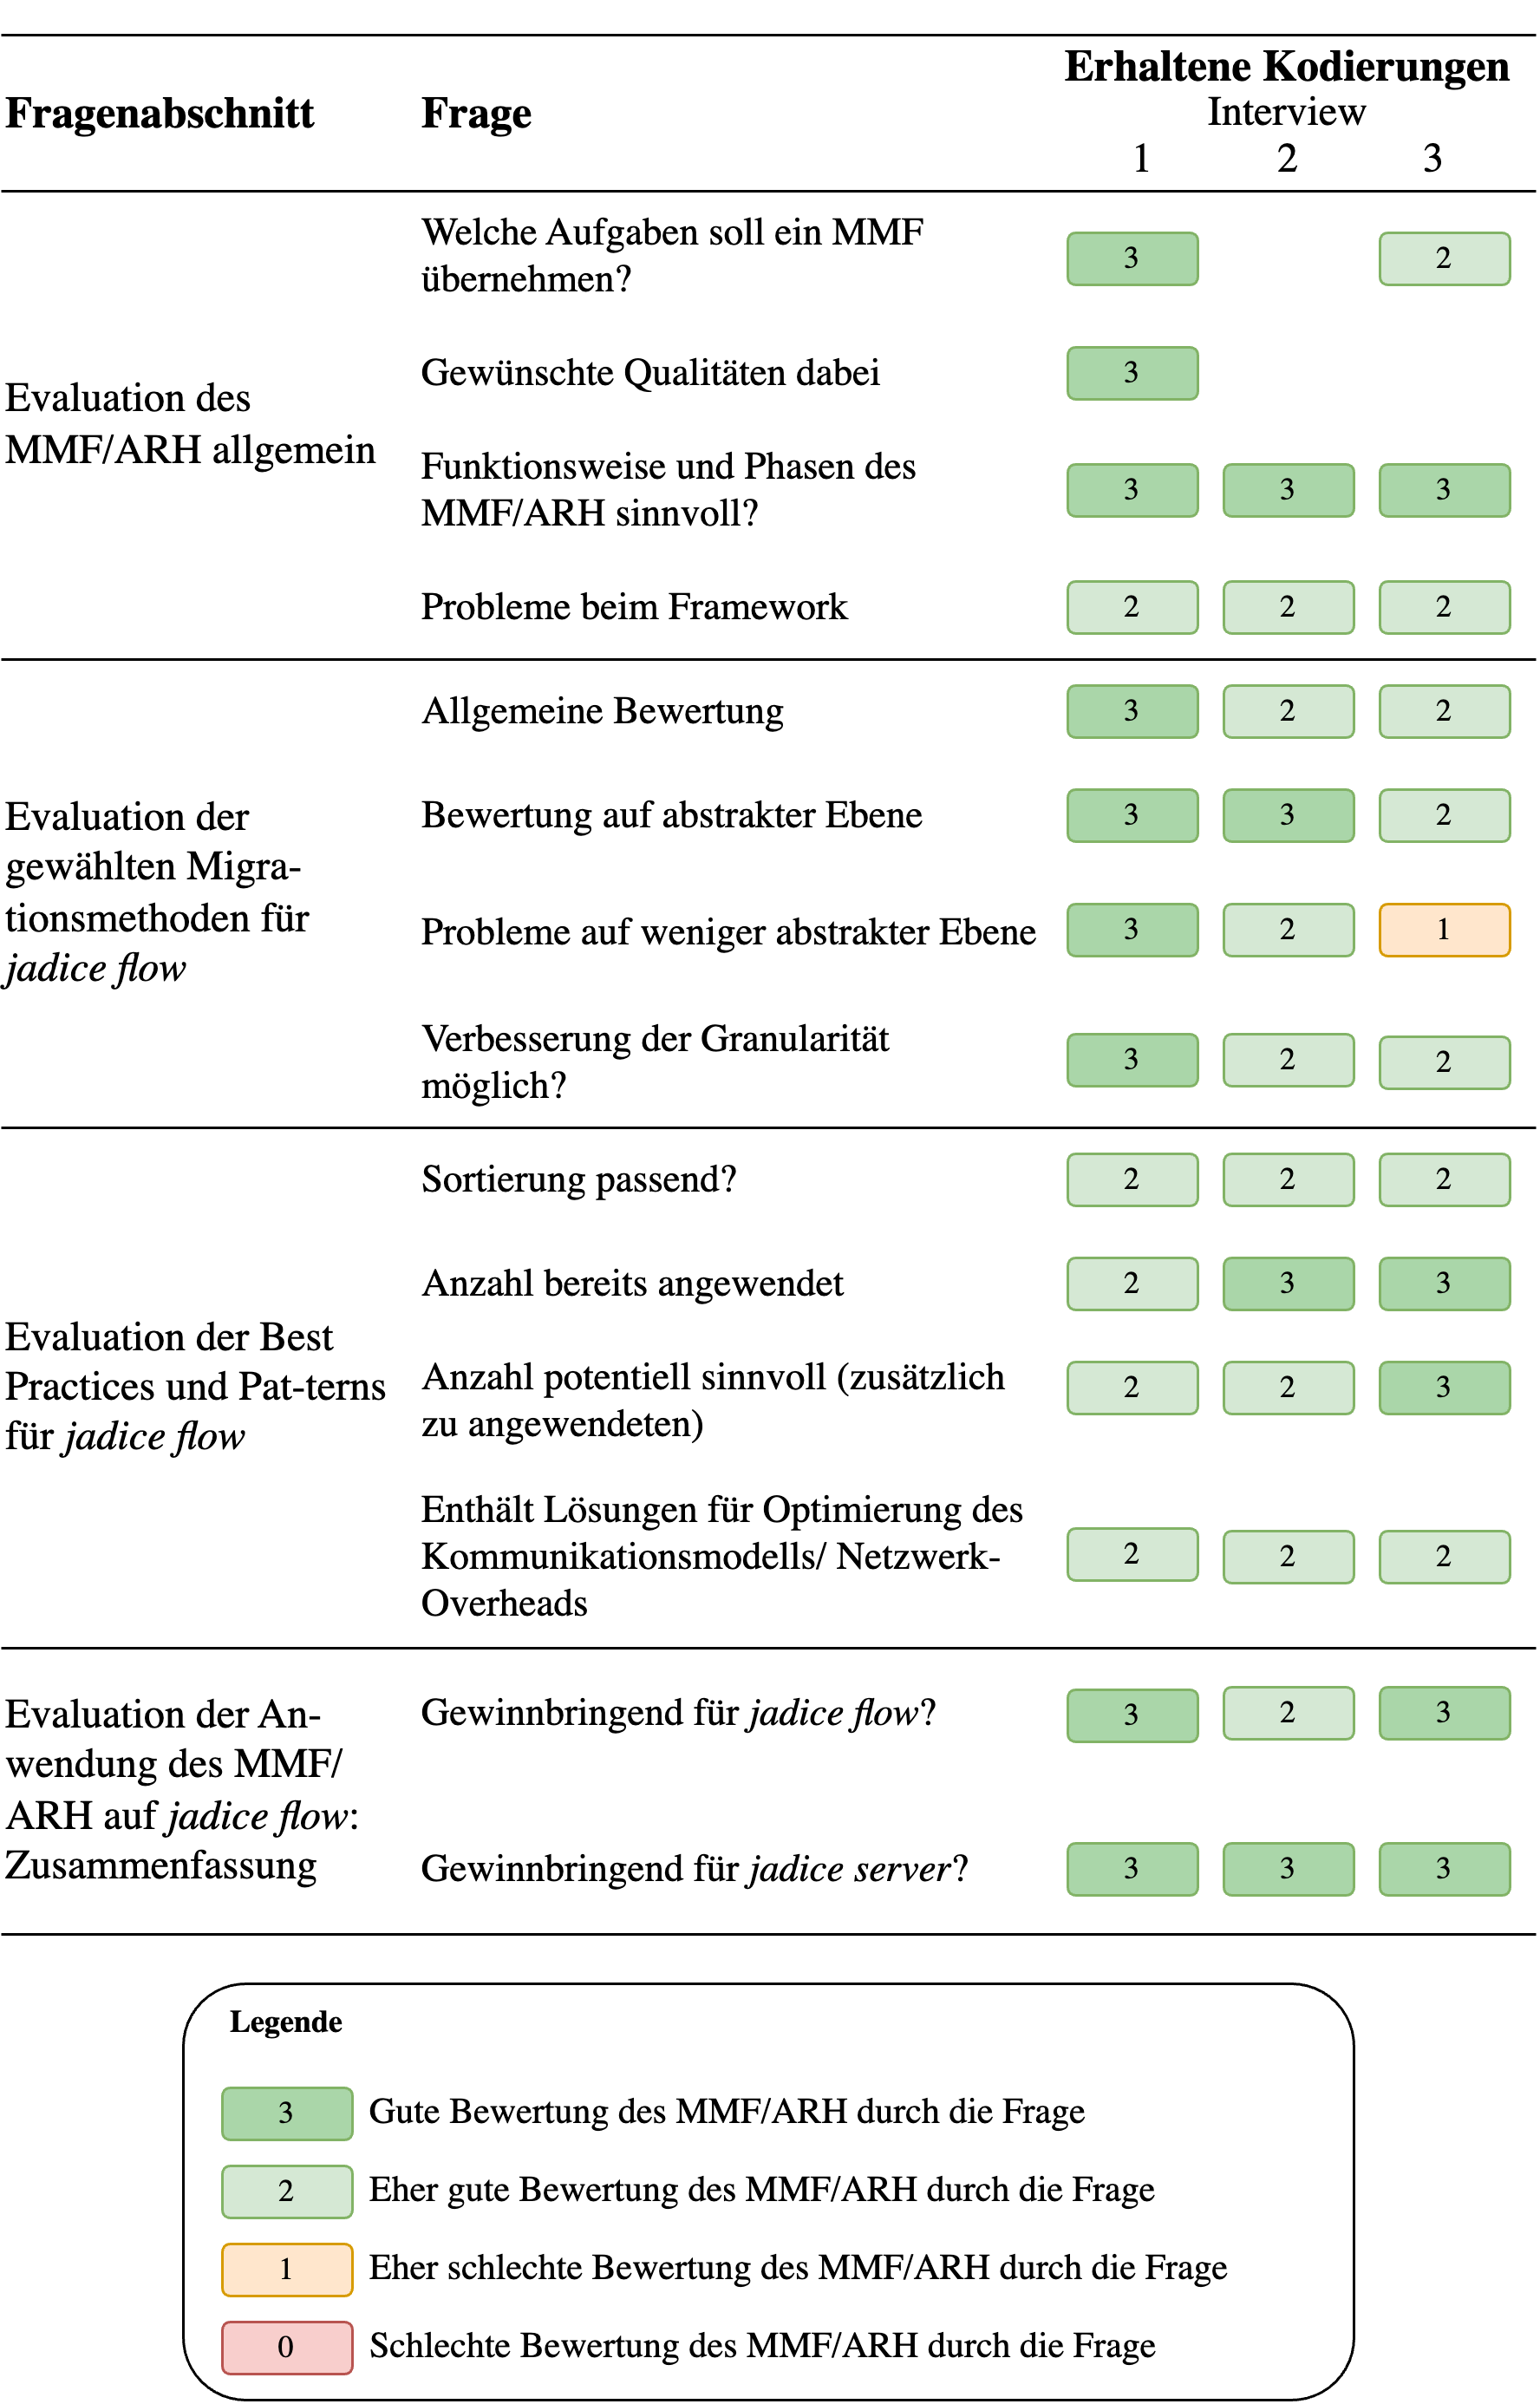
\includegraphics[width=0.8\textwidth]{interview-kodierung-auswertung.drawio}
	\caption[Auswertung Kodierung Experteninterviews]{
		Auswertung der Kodierung der Experteninterviews.
	}
	\label{fig:auswertung-interviews-kodierung}
\end{figure}
%Die Fragen der Interviews auf zwei Abschnitte unterteilt, deren Ergebnisse im Folgenden getrennt beschrieben werden.
%In \cref{sec:evaluation-mmf-allgemein} wird die Auswertung der Fragen, die sich auf die Evaluation des \gls{mmf}/\gls{arh} allgemein beziehen, vollzogen.
%Der hauptsächliche Teil der Auswertung findet dann in \cref{sec:evaluation-mmf-anwendung} statt, wo die spezifische Anwendung des Frameworks in Rahmen dieser Arbeit evaluiert wird.


\subsection{Evaluation des MMF/ARH allgemein}
\label{sec:evaluation-mmf-allgemein}

Dieser Teil der Interviews diente der allgemeinen Bewertung des Frameworks und des Tools.
Die Fragen wurden insbesondere ohne Bezug auf die in dieser Arbeit durchgeführte Migration gestellt.
Hierfür wurde ein Zeitrahmen von zehn Minuten vorgesehen, der mit durchschnittlich neun Minuten pro Interview auch eingehalten wurde.

\paragraph{Gewünschte Features eines \gls{mmf}:} In der ersten Frage sollte ohne Bezug zum \gls{mmf} oder \gls{arh} untersucht werden, welche Aufgaben ein \acrlong{mmf} allgemein für Entwickler bei der Migration von Monolithen zu Microservices übernehmen könnte.
Das Ziel ist es, die Antworten mit den tatsächlichen Funktionen des \gls{arh} abzugleichen und ggf. Ideen für zukünftige Funktionen des \gls{arh} zu sammeln.
In den Interviews hat sich herausgestellt, dass die Frage schwer verständlich ist, da zwei von drei Teilnehmern oft Konzepte eines Meta-Frameworks wie dem \gls{arh} mit konkreten Migrationsverfahren vermischt haben.
In einem Interview wurde daher die Frage schlussendlich übersprungen, da auch eine Wiederholung und Vertiefung der Frage keine Antwort erbrachte.
In nur einem Interview wurde die Frage hinreichend verstanden und beantwortet, um sinnvoll die damit verknüpfte zweite Frage stellen zu können.
Diese wurde in den anderen beiden Fällen schlicht übersprungen.

Zu großen Teilen wurden in den Antworten auf die erste Frage Funktionen genannt, die der \gls{arh} anbietet.
Dazu gehören das Sammeln von Informationen und die Definition von Anforderungen (umgesetzt in Phase 1)  sowie die Suche nach Verfahren durch die primär die Granularität der Microservices optimiert werden kann (umgesetzt in Phase 2).
Als gewünschte Qualität wurde dabei genannt, dass eine große Auswahl an Verfahren bevorzugt wird, von denen dann mehrere manuell verglichen werden können.
Weitere Ideen sind die Visualisierung der gesammelten Informationen, ein Teilen der Informationen, um besser im Team arbeiten zu können und Tipps für den Migrationsprozess.
Letzteres könnte als teilweise umgesetzt bewertet werden, da das gesamte Framework als Leitfaden für die Migration gesehen werden kann.
Generell ist die Aussagekraft dieses Fragenabschnittes dadurch eingeschränkt, dass die Teilnehmer im Vorfeld über die Funktionsweise des \gls{arh} informiert wurden und somit diese Fragen nicht mehr völlig unbeeinflusst beantworten konnten.

\paragraph{Funktionsweise des \gls{mmf}:} Anschließend folgen Fragen zur Bewertung der generellen Funk\-ti\-ons\-wei\-se des \gls{mmf} in Phasen.
Alle Experten haben angegeben, dass sie die Phasenaufteilung als sinnvoll ansehen.
Dass Phase 1 eine Analyse des Systems und die Planung der Ziele durchgeführt wird, wurde als sehr natürlich für allgemeine Refactoringprozesse wahrgenommen.
Vorschläge von Migrationsverfahren in der zweiten Phase wurden ebenfalls als positiv bewertet.
Es wird vermutet, dass so Verfahren gefunden werden können, die sonst nicht betrachtet worden wären.
Das Zusammenspiel der Phasen wurde ebenfalls als sinnvoll bewertet.
Es würde eine stetige Evaluierung der gewählten Vorgehensweise begünstigt und angestoßen werden.

\paragraph{Probleme des \gls{mmf}/\gls{arh}:} Auf die Frage nach Problemen am \gls{mmf} oder \gls{arh} wurden einige potentielle Probleme identifiziert.
Ein Teilnehmer kritisierte die Dokumentation des \gls{arh}. 
Ein Beispiel dafür sei die Beschreibung der Filteroptionen für die Suche nach Migrationsverfahren.
Diese Kritik wurde vom Teilnehmer selbst direkt im Bezug auf das junge Entwicklungsstadium des Werkzeugs und die wissenschaftliche Orientierung relativiert.
Außerdem wurde von einem Experten hervorgehoben, dass der Haupteinflussfaktor auf die Nützlichkeit des Werkzeugs die Datenbasis ist, die verfügbar ist.
Diese müsse stetig aktualisiert und gut kategorisiert werden.
Eine weitere Kritik bezieht sich auf die Einschränkung auf bestimmte \glspl{qa} in der ersten Phase.
Da die verfügbaren \glspl{qa} auch in der Kategorisierung der Verfahren vorhanden sein müssen, ist das Modell nicht erweiterbar und bildet möglicherweise in bestimmten Anwendungsfällen nicht die nötigen Anforderungen ab.
Die Schwere dieser Kritiken wurde sowohl von den Teilnehmern als auch vom Autor als relativ gering eingeschätzt.

\subsection{Evaluation der Anwendung des MMF/ARH auf \jf}
\label{sec:evaluation-mmf-anwendung}

Während im ersten Teil der Fragen der Fokus auf der allgemeinen Funktionsweise des \gls{mmf} und \gls{arh} lag, wurde in diesem Teil ein Bezug zu der in dieser Arbeit durchgeführten Anwendung des Frameworks auf \jf hergestellt.
Dafür wurden erst Fragen zu zwei ausgewählten Migrationsmethoden und dann zu der Liste von \bpp, die der \gls{arh} für \jf anbietet, gestellt.
Als Hauptteil wurde in diesem Abschnitt der Interviews die größte Dauer vermutet, jedoch mit 20 Minuten trotzdem zu gering kalkuliert.
In nur einem Interview konnte diese Zeitspanne eingehalten werden, im Durchschnitt benötigte dieser Abschnitt 27 Minuten.
Vor allem die Befragung zu den \bpp dauerte mit durchschnittlich 14 Minuten länger als erwartet.
Durch das Einhalten des allgemeinen Zeitrahmens stellt das jedoch kein Problem dar.

\subsubsection{Evaluation der ausgewählten Migrationsmethoden für \jf}
\label{sec:evaluation-mmf-anwendung-methoden}

In diesem Fragenabschnitt wurden den Teilnehmern Fragen zu den ausgewählten Mi\-gra\-ti\-ons\-ver\-fah\-ren gestellt.
Diese wurden vor Beginn der ersten inhaltlichen Fragen im Rahmen der Verständnisfragen (siehe \cref{sec:verständnisfragen}) mit den Teilnehmern besprochen, um sicherzustellen, dass das Verständnis der Verfahren für eine Bewertung dieser ausreicht.
Im Folgenden werden die Verfahren auf Basis ihrer Reihenfolge im Informationsmaterial in \cref{chap:expert-interviews-infobogen} referenziert.
Verfahren 1 entspricht demnach \result{2} und Verfahren 2 \result{3}.
Als Einstieg dieses Teils wurde eine allgemeine Bewertung der Nützlichkeit der Verfahren im Bezug auf \jf abgefragt.
Oft wurden dadurch die folgenden Fragen zur Bewertung auf abstrakter und auf weniger abstrakter, technischer Ebene bereits teilweise beantwortet.

\paragraph{Abstrakte Funktionsweise:} Auf abstrakter Ebene wurden beide Verfahren von allen Teilnehmern als potentiell geeignet bewertet.
Vor allem die Art der Eingabe(n) und Ausgaben der Verfahren stand bei den Antworten im Fokus.
Ein Experte favorisierte das zweite vor dem ersten Verfahren, die anderen beiden umgekehrt.
Als Grund für die Bevorzugung des  zweiten Verfahrens wurde die besser passende Eingabe einer bereits vorhandenen \gls{msa} sowie die Visualisierung der Metriken für eine manuelle Überarbeitung der Architektur genannt.
Diese wird zusätzlich zur Optimierung der Serviceaufteilung mit einem Algorithmus, die auch das zweite Verfahren beinhaltet, angeboten.
Die anderen Experten bewerteten diese Vorteile des ersten Verfahrens als weniger wichtig und gaben an, dass sie die Eingabe in Form von einem \gls{bpmn}-Diagramm den User Stories vorziehen würden.
Das liegt vor allem daran, dass die User Stories eine weniger technische Ebene abbilden und damit schwerer greifbar ist, wie die Verbindung zwischen verschiedenen Einheiten analysiert und die Architektur verbessert werden soll.
Sie evaluierten die zweite Methode dennoch als potentiell sinnvoll anwendbar, nur eben als Ergänzung zur ersten Methode.

\paragraph{Technische Ebene:} Auf abstrakter Ebenen kann ein Konzept sinnvoll klingen und in der Realität trotzdem nicht funktionieren.
Deshalb wurde gefragt, ob die Experten sich konkrete Probleme bei der Umsetzung der Verfahren vorstellen können.
Hierbei muss beachtet werden, dass die Antwortmöglichkeiten der Experten bei der Frage sehr beschränkt sind, da sie die Verfahren nicht im Detail kennen.
Selbst bei besserer Informationslage über die Verfahren kann es passieren, dass bestimmte Probleme erst in der Praxis auffallen.
Die Evaluation dieser Frage soll deshalb nicht als Beweis für das sichere Gelingen der Verfahren in einer Anwendung mit \jf dienen, sondern nur beleuchten, ob die Verfahren schon bei anfänglicher Betrachtung Probleme aufwerfen, die den Versuch einer Anwendung infrage stellen.

Insgesamt wurden auf diese Frage wenige Probleme von den Experten genannt.
Ein Experte sah gar keine Probleme und konnte auf die kritische Nachfrage des Interviewers, der ein potentielles Problem benannte, sinnvoll argumentieren, dass er dieses nicht als Problem sieht.
Die anderen Experten nannten einige Probleme, von denen sie aber keines als zu kritisch für eine Anwendung der Verfahren einschätzten.
Unter anderem wurde für die Eingabe von \gls{bpmn}-Diagrammen argumentiert, dass man \glqq nur das bekommt, was man hereingibt\grqq{}.
Damit wird kritisiert, dass manuell erstellte Eingaben nicht objektiv sind und diese Subjektivität das Ergebnis beeinflussen kann.
Außerdem merkte ein anderer Experte allgemeiner an, dass nie komplett vollständige Eingabedaten vorliegen und durch fehlende Daten unvorhergesehene Probleme entstehen können.
Als Beispiel wurden \emph{Edge Cases} genannt, die womöglich nicht vom Verfahren berücksichtigt werden können, aber einen großen Einfluss auf den Erfolg einer Architektur haben können.

\paragraph{Bezug zur Forschungsfrage:} Abschließend zu den Verfahren wurde jeweils die Frage gestellt, ob summa summarum eine Anwendung der Verfahren als potentiell gewinnbringend im Bezug auf die Granularität der Microservices von \jf erachtet wird.
Da die Frage sehr hypothetisch ist, waren sich einige Teilnehmer etwas unsicher, insgesamt wurde aber von zwei Teilnehmern eine positive Tendenz verzeichnet und vom anderen Teilnehmer ein klares \glqq Ja\grqq{}.


\subsubsection{Evaluation der \bpp für \jf}
\label{sec:evaluation-mmf-anwendung-bp-patterns}

Als ebenfalls wichtiger Bestandteil des Frameworks wurde in den Interviews auch konkreter zur dritten Phase befragt.
Da im Gegensatz zu den Migrationsverfahren die Namen von \bpp in vielen Fällen genug Aussagekraft haben, damit die Teilnehmer das Konzept verstehen, wurde hier keine Vorselektion getroffen, sondern alle Einträge des \gls{arh} den Teilnehmern gezeigt.
Dabei ist klar, dass den Experten nicht alle Ansätze im Voraus bekannt sind oder durch den Namen klar werden.
Die einzige zeitlich sinnvolle Lösung dafür ist, alle nicht verstandenen \bpp zu ignorieren, was den Experten so auch gesagt wurde.
Das Ziel dieses Teils ist dabei die Bewertung der Experten, ob das Werkzeug für Findung und Wahl von passenden \bpp zielführend ist und auch einen Vorteil gegenüber manueller Recherche bieten kann.

\paragraph{Ordnung der Ergebnisse:} Im ersten Schritt sollten die Experten die Sortierung der \bpp bewerten.
Dabei wurde hervorgehoben, dass diese auf Basis der \glspl{qa} \emph{Scalability}, \emph{Maintainability}, \emph{Performance} und \emph{Portability} entsteht.
Die Sortierung wurde grundlegend von allen Teilnehmern als sinnvoll bewertet.
An wenigen Stellen wurden Ergebnisse in einer anderen Priorisierung eingeschätzt, größtenteils wurden dabei aber Einwände wieder relativiert, nachdem erneut über die eingegebenen \glspl{qa} nachgedacht wurde.
Ein Teilnehmer erwähnte auch, dass man mit anderer Erwartungshaltung an diese Liste herangehen sollte, als beispielsweise an die Liste der Migrationsverfahren.
Das liegt daran, dass sich nicht auf einzelne \bpp festgelegt werden muss, sondern mehrere kombinierbar sind.
Es wurde speziell hervorgehoben, dass auch zum Beispiel manche Ergebnisse mit nur einer Übereinstimmung gewinnbringend sein können, wenn sie für ein bestimmtes \gls{qa} sehr gut sind, aber kein anderes bedienen.

\paragraph{Bereits umgesetzte und potentiell sinnvolle \bpp:}
Als nächstes wurden die Einschätzungen der Experten zu der Anzahl der bereits in \jf umgesetzten \bpp sowie zu den noch nicht umgesetzten, aber potentiell sinnvollen, abgefragt.
Vom Interviewer wurde explizit angemerkt, dass lediglich eine Einschätzung abgegeben werden werden soll und Ergebnisse mit unbekannten Namen ignoriert werden sollen.
Im Durchschnitt wurde eingeschätzt, dass 13 Patterns und 15 Best Practices bereits in \jf (teilweise) umgesetzt sind und  5 Patterns sowie 4 Best Practices für die zukünftige Implementierung potentiell sinnvoll wären.
Die Abweichung der Antworten war dabei sehr hoch, vermutlich aufgrund der spekulativen Fragestellung. 
Eine Einschätzung ist schwierig, wenn lediglich die Namen der Ergebnisse betrachtet werden.
Ein vorsichtiger Teilnehmer, der keine falschen Ergebnisse mit einschließen will, könnte zu geringeren Zahlen kommen als ein selbstsicherer, optimistischer Teilnehmer.
Außerdem wurde die Anweisung, nur eine grobe Einschätzung abzugeben und nicht eine knapp 100 Ergebnisse lange Liste genau zu betrachten, unterschiedlich ernst genommen.
Dabei wurde beobachtet, dass der Teilnehmer mit der größten Abweichung deutlich schneller geantwortet hat.
Des Weiteren war bei diesen Antworten auffällig, dass in Prozentanteil von der Gesamtergebnisanzahl (beispielsweise \glqq 60\% der Patterns\grqq{}) geantwortet wurde statt in absoluten Zahlen.
Das könnte auf eine erhöhte Ungenauigkeit der Einschätzung dieses Teilnehmers hindeuten.

\paragraph{Bezug zur Forschungsfrage:} Abschließend wurde gefragt, ob eine Verbesserung des Kom\-mu\-ni\-ka\-ti\-ons\-mo\-dells beziehungsweise des Netzwerk-Overheads durch die \bpp der Liste für möglich gehalten wird.
Die Resonanz dabei war positiv, aber nicht übermäßig positiv.
Es wurden von den Experten jeweils ein bis zwei Möglichkeiten genannt, aber auch betont, dass die Zahl der dafür geeigneten Ergebnisse relativ gering ist und diese Ergebnisse in der Liste nicht hoch priorisiert sind.
Ein Experte erwähnte allerdings auch, dass die \glspl{qa} nicht unbedingt auf dieses Ziel ausgerichtet wurden und dadurch vermutlich diese Sortierung zustande kommt.

\subsubsection{Evaluation der Anwendung des \gls{mmf}/\gls{arh} auf \jf insgesamt}
\label{sec:evaluation-mmf-anwendung-insgesamt}

Zum Abschluss der Interviews wurden jeweils zwei Fragen gestellt, die die Ergebnisse aller vor\-he\-ri\-gen Fragen aggregieren sollten.
Es sollte insgesamt eingeschätzt werden, ob die Verwendung des Frameworks und des Werkzeugs zum momentanen Zeitpunkt gewinnbringend für \jf wäre.
Dieselbe Frage wurde anschließend im Bezug auf das Vorgängerprodukt mit monolithischer Architektur eine Verwendung in der Vergangenheit wiederholt.

Zwei der Teilnehmer bewerteten die Verwendung zum jetzigen Zeitpunkt als sinnvoll.
Der andere Teilnehmer war unsicherer, tendierte jedoch auch dazu.
Alle waren sich darin einig, dass eine Anwendung für die Migration in der Vergangenheit noch wertvoller gewesen wäre.
Ein Experte war unsicher, ob die Verwendung des \gls{mmf} neues Optimierungspotenzial aufzeigt, das noch nicht bekannt ist.
Die Liste von \bpp sei zwar eine schöne Übersicht, aber wirklich neue Ansätze hätte er nicht gesehen.
Ein anderer Experte hob dagegen hervor, dass das Werkzeug eine gute Übersicht für Architekten bietet und neue Anregungen fördert.
Bei diesen Meinungsverschiedenheiten der Experten konnte eine leichte Korrelation zwischen einer höheren Berufserfahrung der Experten und einer besseren Gesamtbewertung des Frameworks festgestellt werden.
Die Aussagekraft dieses Ergebnisses sollte aufgrund der geringen Teilnehmerzahl jedoch nicht überbewertet werden.

\section{Feldnotizen}
\label{sec:auswertung-feldnotizen}

Während der Anwendung des Frameworks auf \jf in dieser Arbeit wurden in den Phasen 2 und 3 strukturierte Feldnotizen erstellt, die wichtige Schritte dieser Phasen festhalten.
Die Methodik für die Erstellung der Feldnotizen ist in \cref{sec:structured-field-notes} beschrieben.
In diesem Abschnitt wird die Auswertung dieser Feldnotizen mit der in \cref{sec:methodik-auswertung-feldnotizen} erläuterten Codierung  durchgeführt.

Insgesamt wurden 18 Feldnotizen erstellt, wovon 14 in die zweite Phase und vier in die dritte Phase des \gls{mmf} fallen.
In Phase 1 wurden keine Feldnotizen formuliert.
Aufgrund der großen Anzahl von Feldnotizen in der zweiten Phase wurde die Phase für die Auswertung weiter in die übergeordneten Schritte \emph{Filterwahl} mit den \cref{feldnotiz:1,feldnotiz:2,feldnotiz:3} und \emph{Ergebnisbetrachtung} mit den \cref{feldnotiz:4,feldnotiz:5,feldnotiz:6,feldnotiz:7,feldnotiz:8,feldnotiz:9,feldnotiz:10,feldnotiz:11,feldnotiz:12,feldnotiz:13,feldnotiz:14} unterteilt.
Im Folgenden wird die Auswertung der zugehörigen Feldnotizen für jeden dieser Schritte beschrieben.

\subsection{Phase 2: Filterwahl}

In diesem Schritt wurden die Filter für die Suche nach Migrationsverfahren ausgewählt.
Die Entscheidungen dafür wurden ausschließlich in Besprechungen zwischen dem Autor und dem \gls{po} von \jf oder dem universitären Betreuer getroffen.
Dabei wurden drei Feldnotizen erstellt, deren Auswertung durch die festgelegte Kodierung in \cref{tab:auswertung-feldnotizen-1} zu sehen ist.

\begin{table}[!ht]
  \centering
  \begin{tabular}{m{2.8cm} | c c c | c}
    \toprule
    \multirow{2}{*}[0cm]{\textbf{Code}} & \multicolumn{3}{c|}{\textbf{Feldnotiz}} & \multirow{2}{*}[0cm]{\textbf{Summe} (3)} \\
     & \textbf{\fn{1}} & \textbf{\fn{2}} & \textbf{\fn{3}} & \\ \midrule
    Gut gelaufen                        & \checkmark & \checkmark & \checkmark & 3 (100\%)  \\ \hline
    Schlecht gelaufen                   & \checkmark &                       & & 1 (33\%)  \\ \hline
    Mehr gut gelaufen                   & \checkmark & \checkmark & \checkmark & 3 (100\%)  \\ \hline
    Mehr schlecht \:\:\:\:\:\: gelaufen & &                                  & & 0 (0\%)    \\ \hline
    Gutes Gefühl                        & & \checkmark & \checkmark            & 2 (67\%)   \\ \hline
    Schlechtes Gefühl                   & \checkmark & &                       & 1 (33\%)   \\
    Unsicherheit                        & \checkmark & &                       & 1 (33\%)   \\
    Frustration                         & & &                                  & 0 (0\%)    \\ \hline
    Verbesserungs\-vorschlag            & \checkmark & &                       & 1 (33\%)   \\ \hline
    Einzelarbeit                        & & &                                  & 0 (0\%)    \\ \hline
    Besprechung                         & \checkmark & \checkmark & \checkmark & 3 (100\%) \\
    \bottomrule
  \end{tabular}
  \caption[Auswertung Kodierung Feldnotizen Filterwahl]{
    Auswertung der Kodierung der Feldnotizen in Phase 2 beim übergeordneten Schritt \emph{Filterwahl}.
    Prozentuale Angaben hinter der Summe beziehen sich auf den Anteil des Auftreten des Codes zu der Anzahl der Feldnotizen.
  }
  \label{tab:auswertung-feldnotizen-1}
\end{table}


Wie in der Tabelle erkennbar ist, verlief dieser Schritt sehr positiv.
In jeder Feldnotiz wurde eine Sache vermerkt, die gut gelaufen ist und nur in einem Fall ein Problem.
Das ist auch an der Häufigkeit von 100 Prozent der Kodierung \glqq Mehr gut gelaufen\grqq{} zu sehen.

In den Einträgen der Empfindungen ist zu erkennen, dass trotz des positiven Verlaufs dieses Schritts ein Mal auch das schlechte Gefühl \glqq Unsicherheit\grqq{} festgehalten wurde.
Das hängt in diesem Fall jedoch nicht mit dem \gls{arh} oder der Migration zusammen, sondern wird auf die Unerfahrenheit des Autors mit der Anwendung der Methodik von Feldnotizen zurückgeführt.
Ansonsten wurde in 67 Prozent der Feldnotizen ein positives Gefühl vermerkt.
Zudem wurde ein Verbesserungsvorschlag kodiert, der direkt mit der Kodierung \glqq Schlecht gelaufen\grqq{} der \cref{feldnotiz:1} zusammenhängt.
Es wird die Beschreibung der Filteroptionen bemängelt.
Da der \gls{arh} noch in der Entwicklung ist, sind Mängel in der Dokumentation zu erwarten.

\subsection{Phase 2: Betrachtung der Filterergebnisse}

In diesem Schritt wurde mithilfe der im vorherigen Schritt gesammelten Filter eine Suche nach Migrationsverfahren durchgeführt.
Für jedes der acht in Einzelarbeit betrachteten Verfahren wurde je eine Feldnotiz erstellt.
Außerdem wurden drei Feldnotizen bei Besprechungen über die Bewertung der Verfahren für \jf erstellt.
Die Kodierung dieser ist in \cref{tab:auswertung-feldnotizen-2} zu sehen.

\begin{table}[!ht]
  \centering
  \begin{tabular}{m{2.8cm} | c c c c c c c c c c c | c}
    \toprule
    \multirow{2}{*}[0cm]{\textbf{Code}} & \multicolumn{11}{c|}{\textbf{Feldnotiz}} & \multirow{2}{*}[0cm]{\textbf{Summe} (11)} \\
     & \textbf{\fn{4}} & \textbf{\fn{5}} & \textbf{\fn{6}} & \textbf{\fn{7}} & \textbf{\fn{8}} & \textbf{\fn{9}} & \textbf{\fn{10}} & \textbf{\fn{11}} & \textbf{\fn{12}} & \textbf{\fn{13}} & \textbf{\fn{14}} & \\ \midrule
    Gut gelaufen                        & & \checkmark & \checkmark & \checkmark & & \checkmark & & \checkmark & \checkmark & \checkmark & \checkmark & 8 (73\%) \\ \hline
    Schlecht gelaufen                   & \checkmark & & & & \checkmark & \checkmark & \checkmark & & \checkmark & \checkmark & \checkmark            & 7 (64\%) \\ \hline
    Mehr gut gelaufen                   & & \checkmark & \checkmark & \checkmark & & & & \checkmark & & &                                             & 4 (36\%) \\ \hline
    Mehr schlecht \:\:\:\:\:\: gelaufen & \checkmark & & & & \checkmark & & & & & &                                                                   & 2 (18\%) \\ \hline
    Gutes Gefühl                        & & \checkmark & \checkmark & & & & & & & &                                                                   & 2 (18\%) \\ \hline
    Schlechtes Gefühl                   & \checkmark & & & & & & & & & & \checkmark                                                                   & 2 (18\%) \\
    Unsicherheit                        & & & & & & & & & & & \checkmark                                                                              & 1 (09\%) \\
    Frustration                         & \checkmark & & & & & & & & & &                                                                              & 1 (09\%) \\ \hline
    Verbesserungs\-vorschlag            & \checkmark & & & & & & & & & &                                                                              & 1 (09\%) \\ \hline
    Einzelarbeit                        & \checkmark & \checkmark & \checkmark & & \checkmark & \checkmark & \checkmark & & \checkmark & \checkmark & & 8 (73\%) \\ \hline
    Besprechung                         & & & & \checkmark & & & & \checkmark & & & \checkmark                                                        & 3 (27\%) \\
    \bottomrule
  \end{tabular}
  \caption[Auswertung Kodierung Feldnotizen Ergebnisbetrachtung]{
    Auswertung der Kodierung der Feldnotizen in Phase 2 beim übergeordneten Schritt \emph{Ergebnisbetrachtung}.
    Prozentuale Angaben hinter der Summe beziehen sich auf den Anteil des Auftreten des Codes zu der Anzahl der Feldnotizen.
  }
  \label{tab:auswertung-feldnotizen-2}
\end{table}


Die Ergebnisse dieses Schritts fallen gemischt aus.
In 73 Prozent der Feldnotizen wurden positive Aspekte notiert, jedoch wurden in fast genauso vielen Feldnotizen (64 Prozent) auch negative Aspekte festgehalten.
Durch \glqq Gut gelaufen\grqq{} und \glqq Schlecht gelaufen\grqq{} wurde in diesem Schritt bei der Ergebnisbetrachtung der Eindruck von dem jeweiligen Verfahren kodiert.
Bei nur zwei der Feldnotizen der Ergebnisbetrachtung in Einzelarbeit wurde \glqq Gut gelaufen\grqq{} kodiert, ohne dass \glqq Schlecht gelaufen\grqq{} kodiert wurde.
Diese beiden Verfahren wurden für die Phase 3 ausgewählt.
Letztendlich wurde jedoch doppelt so oft \glqq Mehr gut gelaufen\grqq{} kodiert wie \glqq Mehr schlecht gelaufen\grqq{}.
Der Schritt kann daher trotz gewisser Schwierigkeiten als größtenteils positiv verlaufen interpretiert werden.
In den Besprechungen wurde früh festgestellt, dass die Ergebnisse Optionen enthalten, deren Anwendung potentiell möglich ist.
Das spiegelt sich auch darin wider, dass in 67 Prozent der Besprechungen mehr gut gelaufen ist und nur in einem Fall gleich viel gut wie schlecht gelaufen ist.
Die große Anzahl der Kodierungen von \glqq Schlecht gelaufen\grqq{} hängt größtenteils mit Verfahren zusammen, die sich weniger gut für die Anwendung an \jf eignen.
Jedoch ist auch von anderen Suchmaschinen bekannt, dass nicht alle Suchergebnisse zur Vorstellung des Suchenden passen.
In der Praxis wird sich jedoch vermutlich zeigen, dass es genügt, ein bis zwei passende Verfahren mit \gls{arh} zu finden zu und diese zu verwenden.
Eine größere Auswahl an passenden Verfahren wäre dennoch wünschenswert.
Allerdings ist es aufgrund des frühen Stadiums des \gls{arh} wahrscheinlich, dass die Auswahl an Verfahren in Zukunft noch erweitert wird.
Außerdem bildet die durchgeführte Suche nur die Kriterien ab, die für \jf als sinnvoll befunden wurden.
Die Anzahl der sinnvollen Ergebnisse kann für andere Anwendungsfälle variieren.

Die in diesem Schritt notierten Gefühle sind relativ neutral.
In der ersten Feldnotiz (\cref{feldnotiz:4}) wurde Frustration vermerkt, da das erste Suchergebnis, für welches der \gls{arh} mit Abstand die größte Übereinstimmung angezeigt hat, als ungeeignet befunden wurde.
In der letzten Feldnotiz (\cref{feldnotiz:14}) wurde vermerkt, dass es Unsicherheiten bezüglich der zeitlichen Umsetzbarkeit der beiden ausgewählten Verfahren gibt.
Diese Gefühle überwiegen aber nicht den verzeichneten positiven Gefühlen bei der Betrachtung der zwei favorisierten Verfahren in \cref{feldnotiz:5,feldnotiz:6}.

Der in \cref{feldnotiz:4} notierte Verbesserungsvorschlag bezieht sich auf die Frustration in dieser Feldnotiz.
Es wird vorgeschlagen, eine Filteroption zu implementieren, um unpassende Ergebnisse auszuschließen.

\subsection{Phase 3: Anwendung der Migrationsverfahren}
\label{sec:feldnotizen-auswertung-phase3}

In der dritten Phase des \gls{mmf} wurden lediglich vier Feldnotizen erstellt, da nur ein kleiner Teil der Phase durchgeführt wurde.
Die Umsetzung der Phase 3b wurde frühzeitig ausgeschlossen.
Der Hauptteil der Phase 3a, welcher die Anwendung eines Migrationsverfahrens beinhaltet, konnte aufgrund der zeitlichen Beschränkung einer Thesis und Problemen mit den Verfahren nur teilweise durchgeführt werden.
Da in dieser Thesis nicht bis zur Planung einer neuen Architektur fortgeschritten wurde, wurden auch keine \bpp ausgewählt.

Die vier vorhandenen Feldnotizen beschreiben den Versuch, die beiden als Favoriten identifizierten Migrationsverfahren anzuwenden.
Wie in \cref{tab:auswertung-feldnotizen-3} zu sehen ist, war dieser Versuch nicht erfolgreich.
\begin{table}[!ht]
  \centering
  \begin{tabular}{m{2.8cm} | c c c c | c}
    \toprule
    \multirow{2}{*}[0cm]{\textbf{Code}} & \multicolumn{4}{c|}{\textbf{Feldnotiz}} & \multirow{2}{*}[0cm]{\textbf{Summe} (4)} \\
     & \textbf{\fn{15}} & \textbf{\fn{16}} & \textbf{\fn{17}} & \textbf{\fn{18}} & \\ \midrule
    Gut gelaufen                        &  & \checkmark &  &                                & 1 (25\%)  \\ \hline
    Schlecht gelaufen                   & \checkmark & \checkmark & \checkmark & \checkmark & 4 (100\%) \\ \hline
    Mehr gut gelaufen                   &  &  &  &                                          & 0 (0\%)   \\ \hline
    Mehr schlecht \:\:\:\:\:\: gelaufen & \checkmark & \checkmark & \checkmark & \checkmark & 3 (75\%)  \\ \hline
    Gutes Gefühl                        &  &  &  &                                          & 0 (0\%)   \\ \hline
    Schlechtes Gefühl                   & \checkmark & \checkmark & \checkmark & \checkmark & 4 (100\%) \\
    Unsicherheit                        &  & \checkmark &  &                                & 1 (25\%)  \\
    Frustration                         & \checkmark &  & \checkmark & \checkmark           & 3 (75\%)  \\ \hline
    Verbesserungs\-vorschlag            &  &  &  &                                          & 0 (0\%)   \\ \hline
    Einzelarbeit                        & \checkmark & \checkmark & \checkmark &            & 3 (75\%)  \\ \hline
    Besprechung                         &  &  &  & \checkmark                               & 1 (25\%)  \\
    \bottomrule
  \end{tabular}
  \caption[Auswertung Kodierung Feldnotizen Methodenanwendung]{
    Auswertung der Kodierung der Feldnotizen in Phase 3 beim übergeordneten Schritt \emph{Methodenanwendung}.
    Prozentuale Angaben hinter der Summe beziehen sich auf den Anteil des Auftreten des Codes zu der Anzahl der Feldnotizen.
  }
  \label{tab:auswertung-feldnotizen-3}
\end{table}

In nur einer Feldnotiz wurde etwas notiert, das gut gelaufen ist.
Dagegen ist in allen Feldnotizen etwas schlecht gelaufen.
75 Prozent der Notizen wurden mit \glqq Mehr schlecht gelaufen\grqq{} bewertet.
Jede Notiz enthielt ein negatives Gefühl, dreimal Frustration und einmal Unsicherheit.
Ein positives Gefühl wurde nie vermerkt.

Die schlechten Ergebnisse in dieser Phase sind hauptsächlich auf Zeitgründe und die Schwierigkeit bei der Umsetzung der ausgewählten Migrationsverfahren zurückzuführen.
Eine detailliertere Beschreibung der Probleme ist in \cref{sec:anwendung-verfahren} gegeben.
Für die Probleme werden hauptsächlich zwei Quellen vermutet.
Zum einen wurden die Verfahren nur von einer Person im Detail betrachtet und versucht umzusetzen.
Diese Person ist relativ unerfahren, was das Verständnis von wissenschaftlichen Artikeln mit komplexen Algorithmen und Formeln einschränken könnte.
Auf der anderen Seite sind bestimmte Details, zumindest im zweiten Verfahren, wenig ausführlich oder gar nicht beschrieben.
Für eine erfolgreiche Umsetzung dieses Verfahrens wird ein hoher Eigenentwicklungsaufwand eingeschätzt, um den Algorithmus und enthaltene Formeln zu verstehen und umzusetzen.

\subsection{Zusammenfassung}

Nachdem die Ergebnisse der Auswertung der Feldnotizen pro Phase beziehungsweise Schritt in einzelnen Abschnitten beschrieben wurden, wird in diesem Abschnitt aus einer übergeordneten Perspektive auf die Ergebnisse der Feldnotizen geblickt.
Für jeden übergeordneten Schritt wurde die Summe der Kodierung aller enthaltenen Feldnotizen zusammen in der \cref{tab:auswertung-feldnotizen} visualisiert.
\begin{table}[!ht]
  \centering
  \begin{tabular}{m{2.8cm} | M{1cm} m{0.3cm} M{1.8cm} m{0.3cm} M{1.9cm} m{0.3cm} p{0cm} | M{1.8cm}}
    \toprule
    \multirow{2}{*}[-0.3cm]{\textbf{Code}} & \multicolumn{6}{c}{\textbf{Übergeordneter Schritt}} && \multirow{2}{*}[-0.3cm]{\textbf{Summe} (18)} \\
    & \textbf{Filter\-wahl} & \hspace*{-0.2cm}(3) & \textbf{Ergebnis\-betrachtung} & \hspace*{-0.2cm}(11) & \textbf{Methoden\-anwendung} & (4) && \\ \midrule
    Gut gelaufen                        & \mcTwo{3 (100\%)} & \mcTwo{8 (73\%)} & \mcTwo{1 (25\%) } && 12 (67\%) \\ \hline
    Schlecht gelaufen                   & \mcTwo{1 (33\%) } & \mcTwo{7 (64\%)} & \mcTwo{4 (100\%)} && 12 (67\%) \\ \hline
    Mehr gut gelaufen                   & \mcTwo{3 (100\%)} & \mcTwo{4 (36\%)} & \mcTwo{0 (0\%)  } && 7 (39\%) \\ \hline
    Mehr schlecht \:\:\:\:\:\: gelaufen & \mcTwo{0 (0\%)  } & \mcTwo{2 (18\%)} & \mcTwo{3 (75\%) } && 5 (28\%) \\ \hline
    Gutes Gefühl                        & \mcTwo{2 (67\%) } & \mcTwo{2 (18\%)} & \mcTwo{0 (0\%)  } && 4 (22\%) \\ \hline
    Schlechtes Gefühl                   & \mcTwo{1 (33\%) } & \mcTwo{2 (18\%)} & \mcTwo{4 (100\%)} && 7 (39\%) \\
    Unsicherheit                        & \mcTwo{1 (33\%) } & \mcTwo{1 (09\%)} & \mcTwo{1 (25\%) } && 3 (17\%) \\
    Frustration                         & \mcTwo{0 (0\%)  } & \mcTwo{1 (09\%)} & \mcTwo{3 (75\%) } && 4 (22\%) \\ \hline
    Verbesserungs\-vorschlag            & \mcTwo{1 (33\%) } & \mcTwo{1 (09\%)} & \mcTwo{0 (0\%)  } && 2 (11\%) \\ \hline
    Einzelarbeit                        & \mcTwo{0 (0\%)  } & \mcTwo{8 (73\%)} & \mcTwo{3 (75\%) } && 11 (61\%) \\ \hline
    Besprechung                         & \mcTwo{3 (100\%)} & \mcTwo{3 (27\%)} & \mcTwo{1 (25\%) } && 7 (39\%) \\
    \bottomrule
  \end{tabular}
  \caption[Auswertung Kodierung Feldnotizen]{
    Auswertung der Kodierung der Feldnotizen.
    Prozentuale Angaben in Klammern beziehen sich auf den Anteil des Auftretens des Codes zu der Anzahl der Feldnotizen in diesem Schritt beziehungsweise insgesamt.
  }
  \label{tab:auswertung-feldnotizen}
\end{table}


Bei Betrachtung der unterschiedlichen Ergebnisse in den drei Schritten fällt vor allem auf, dass sich die Kodierungen \glqq Mehr schlecht gelaufen\grqq{}/\glqq Mehr gut gelaufen\grqq{} im Verlauf sehr negativ entwickeln.
Im ersten Schritt wurden 100 Prozent mit \glqq Mehr gut gelaufen\grqq{} kodiert, das kehrt sich im letzten Schritt um.
Dort sind 75 Prozent mit \glqq Mehr schlecht gelaufen\grqq{} kodiert.
Dabei lässt sich insbesondere folgendes beobachten: Mit abnehmendem Erfolg der Aktivitäten ist der \gls{arh} immer weniger involviert an den Aktivitäten.
Der erste Schritt befasst sich noch komplett mit dem \gls{arh} und verläuft gut.
Ab dem zweiten Schritt wird die Wertung schlechter und hier ist der \gls{arh} schon weniger involviert.
Obwohl der \gls{arh} die Ergebnisse vorgibt, kann der er nur entfernter mit der Betrachtung der wissenschaftlichen Artikel assoziiert werden.
In der dritten Phase ist die Bewertung dann am schlechtesten, doch die Kritik in der dritten Phase kann fast nur auf die Verfahren bezogen werden und nur in sehr geringem Maße auf den \gls{arh}.

Daraus kann geschlossen werden, dass der \gls{arh} einen Migrationsprozess dort, wo es die Grenzen seiner Funktionsweise es erlauben, gut begleitet.
Es gibt immer Optimierungspotenzial.
Aus der Perspektive dieser Arbeit waren die Verfahren sowie deren etwaige Qualität am kritischsten.
Daher scheint es am wichtigsten, die Sammlung von Verfahren sowie die Bewertung und Kategorisierung dieser zu optimieren.

\section{Diskussion}
\label{sec:auswertung-diskussion}

In diesem Abschnitt wird der gesamte Refactoringprozess, den das \gls{mmf} anleitet und der \gls{arh} umsetzt, bewertet.
Dabei werden die vorangegangenen Auswertungen der Feldnotizen und Experteninterviews zusammengefasst und diskutiert.
Zusätzlich fließt eine qualitative Bewertung des Gesamtprozesses durch den Autor ein, die sich aus den gesammelten Eindrücken ergibt.

Der Migrationsprozess des \gls{arh} bietet folgende wesentlichen Funktionen, die in dieser Arbeit untersucht werden sollen:
\begin{itemize}
	\item Erfassung der \glspl{qa} in Phase 1
	\item Konfiguration der Suchfilter in Phase 2
	\item Suche nach Migrationsverfahren in Phase 2
	\item Suche nach \bpp in Phase 3
\end{itemize}
Die beiden ersten Funktionen produzieren, abgesehen von der \gls{ux} bei der Verwendung der Funktionen, keine eigenen Ergebnisse, die evaluiert werden könnten.
Da sie jedoch die Voraussetzung für die dritte und vierte Funktion sind und deren Ergebnisse beeinflussen, werden sie indirekt durch deren Analyse ausgewertet.

Die Diskussion dieser Funktionen ist nach den Unterfragen der \hyperref[forschungsfrage:1]{Forschungsfrage} gegliedert, da für die Ergebnisse der Phasen 2 und 3 jeweils eine Frage formuliert wurde.

%Eine hypothetisch optimale Filterfunktion würde erreichen, dass Nutzer die Suchergebnisse nach Einstellen seiner Filter hinsichtlich der Nützlichkeit für sein Ziel genau gleich ordnen würde wie der \gls{arh} es tut.
%Natürlich ist eine so genaue Filterfunktion unrealistisch und nicht erreichbar.
%Im Folgenden wird versucht, von den Problemen mit Ergebnissen der Suchen Rückschlüsse auf Probleme in Filterfunktion durch Filter und \glspl{qa} zu ziehen.
%Wenn beispielsweise hoch platzierte Suchergebnisse vom Nutzer als schlecht bewertet werden, könnte ein Zusammenhang mit fehlenden Filtermöglichkeiten oder zu stark bewerteten Filtern bestehen.


\subsection{Forschungsfrage 1.1}
% TODO: erste Phase noch mit rein
Dieser Teil der \hyperref[forschungsfrage:1]{Forschungsfrage} bezieht sich auf die Ergebnisse der zweiten Phase, in der geeignete Migrationsverfahren für \jf untersucht wurden.
Insbesondere wurde dabei die Frage nach einer möglichen Verbesserung der Granularität gestellt.
Sowohl die Feldnotizen als auch die Experteninterviews wurden zur Beantwortung dieser Frage herangezogen.

Die Feldnotizen zeigen, dass die Konfiguration der Filter sehr erfolgreich war und die Suche nach Migrationsverfahren größtenteils positiv verlief.
Der \gls{arh} hat in diesen Phasen wie erwartet funktioniert und nur zu geringfügigen Unsicherheiten geführt, die aufgrund des jungen Entwicklungsstands des Werkzeugs zu erwarten sind.
Wie in \cref{sec:feldnotizen-auswertung-phase3} beschrieben, war die Anwendung der ausgewählten Migrationsverfahren in der dritten Phase weniger erfolgreich.
Es können mehrere Faktoren genannt werden, die zu dieser Situation beitragen.
Die größten sind jedoch der begrenzte zeitliche Rahmen und die Erschwerung der Durchführung der Verfahren in kurzer Zeit aufgrund des Fehlens gewisser Qualitäten der Veröffentlichungen zu den Verfahren.
Die Anwendung von Werkzeug-unterstützten Verfahren wäre grundlegend tendenziell leichter möglich gewesen.
Die Nutzung einer Applikation wird als einfacher und schneller umsetzbar eingeschätzt als die Verwendung eines in einem wissenschaftlichen Artikel beschriebenen Verfahrens.
Beide ausgewählten Verfahren haben ein Werkzeug in dem Artikel vorgestellt, welches aber in beiden Fällen nicht veröffentlicht wurde.
Die Umsetzung des bevorzugten Verfahrens wurde aufgrund seiner zu großen Komplexität in der begrenzten Zeit nicht angestrebt.
Beim zweiten Verfahren wurde eine Anwendung versucht, jedoch nach einiger Zeit abgebrochen.
Einige Details des Algorithmus waren dem Autor unverständlich, da sie nicht ausreichend erklärt wurden.
Diese Probleme traten bei der konkreten Umsetzung auf und waren im Voraus nicht wirklich abschätzbar.
An dieser Stelle wäre es wünschenswert, im \gls{arh} mehr Informationen über die Verfahren zur besser Einschätzung zu erhalten, was in realistischer Abschätzung jedoch auch schwer umsetzbar ist.

Bei der fehlgeschlagenen Anwendung in dieser Thesis ist zu beachten, dass die Ressourcen für die Umsetzung der Verfahren anders begrenzt sind, als es in anderen Anwendungen in der Industrie der Fall wäre.
Die durchgeführten Experteninterviews haben gezeigt, dass die Migrationsverfahren, die durch den \gls{arh} erhalten wurden, als grundsätzlich gut und für die Anwendung mit \jf geeignet eingeschätzt wurden.
Die Experten haben sowohl die beiden vorgestellten Migrationsverfahren als auch ihre spezifische Auswirkung auf die Optimierung der Service-Granularität von \jf als gewinnbringend bewertet.
Die genannten Probleme könnten in Zukunft gelöst und Erfolg erzielt werden, wenn die Anwendung der Verfahren nicht so stark durch Zeit- und Mitarbeiterzahl eingeschränkt wäre.

\subsection{Forschungsfrage 1.2}

Dieser Teil der \hyperref[forschungsfrage:1]{Forschungsfrage} bezieht sich auf die Ergebnisse der dritten Phase, in der geeignete \bpp für \jf gefunden werden sollten.
Insbesondere wurde dabei die Frage nach einer möglichen Verbesserung des Kommunikationsmodells und des damit verbundenen Netzwerk-Overheads gestellt.

Im Gegensatz zur Auswahl eines oder weniger Migrationsverfahren für die Planung einer neuen Architektur können und sollten mehrere \bpp für diese ausgewählt werden.
Als Basis sollte jedoch die in Phase 2 selektierte Migrationsmethode durchgeführt werden und eine neue Architektur vorhanden sein, um sinnvoll adäquate \bpp zu finden und umsetzen zu können.
Da diese Voraussetzung in dieser Arbeit nicht gegeben war, wurde auch die Auswahl von \bpp nicht durchgeführt.

Dieser Teil der  \hyperref[forschungsfrage:1]{Forschungsfrage} kann also nur durch die Ergebnisse der Experteninterviews erörtert werden, da keine Auswahl oder Anwendung von \bpp stattgefunden hat.
Die vier Fragen, die in den Interviews mit Bezug auf die vom \gls{arh} für \jf vorgeschlagenen \bpp gestellt wurden, haben folgende Ergebnisse gezeigt.
Die Experten bewerteten die Sortierung der \bpp im Verhältnis zu den eingegebenen \glspl{qa} größtenteils als sinnvoll.
Außerdem stellten sie fest, dass bereits etwa 13 Patterns und 15 Best Practices in \jf implementiert sind und dass es zusätzlich sinnvoll sein könnte, in Zukunft weitere 5 Patterns und 4 Best Practices zu implementieren.
Dies ist ein Hinweis darauf, dass das Tool eine gute Auswahl an \bpp bietet und dass diese Funktion zumindest im konkreten Anwendungsfall als sinnvoll erachtet werden kann.

Darüber hinaus wurde festgestellt, dass die Liste der \bpp einige Vorschläge enthält, die das Kommunikationsmodell und den damit verbundenen Netzwerk-Overhead von \jf verbessern könnten.
An dieser Stelle haben zwei Experten angemerkt, dass eine Erweiterung der Auswahl an \bpp wünschenswert wäre, da die Anzahl der für diese Frage nützlichen Ergebnisse als gering eingeschätzt wurde.

Es ist jedoch zu beachten, dass der in der \hyperref[forschungsfrage:1]{Forschungsfrage} erwähnte Weg zur Verbesserung des Kommunikationsmodells und des damit verbundenen Netzwerk-Overheads durch \bpp nicht der einzige Weg zum genannten Ziel ist.
Eine Veränderung der Granularität durch ein in Phase 2 gewähltes Verfahren könnte zu einer stark veränderten Kommunikation führen und eine Optimierung des Netzwerk-Overheads ermöglichen.
Ein Beispiel hierfür wäre die Vergrößerung der Microservices.
Dadurch würde die Kommunikation zwischen vorher verschiedenen Microservices nun im selben Microservice stattfinden und müsste nicht mehr über das Netzwerk laufen.

%\subsection{Qualitative Bewertung des Refactoringprozesses}
%
%%Zu Beginn wird eine qualitative Bewertung des Gesamtprozesses vom Autor vorgenommen.
%%Diese kann subjektiv sein und soll daher nur als erste Orientierung dienen und durch Experteninterviews unterstützt werden.
%
%
%Die Auswertung dieser Arbeit durch die Feldnotizen und Experteninterviews ist aufschlussreich, aber deckt nicht den vollen Detailgrad der in dieser Arbeit gemachten Erfahrungen ab.
%In diesem Abschnitt soll der gesamte Refactoringprozess, den das \gls{mmf} leitet, bewertet werden.
%Dabei werden die einzelnen Funktionen des \gls{arh} qualitativ evaluiert.
%Der Prozess besteht aus den folgenden wesentlichen Funktionen:
%\begin{itemize}
%	\item Erfassen der \glspl{qa} in Phase 1
%	\item Einstellen von Suchfiltern in Phase 2
%	\item Suche nach Migrationsverfahren in Phase 2
%	\item Suche nach Patterns und Best Practices in Phase 3
%\end{itemize}
%
%Diese Qualität dieser Funktionen kann über die Ergebnisse der Suchen ausgewertet werden, da die ersten beiden Punkte in die Ergebnisse der letzten beiden Punkte einfließen.
%Eine hypothetisch optimale Filterfunktion würde erreichen, dass Nutzer die Suchergebnisse nach Einstellen seiner Filter hinsichtlich der Nützlichkeit für sein Ziel genau gleich ordnen würde wie der \gls{arh} es tut.
%Natürlich ist eine so genaue Filterfunktion unrealistisch und nicht erreichbar.
%Im Folgenden wird versucht, von den Problemen mit Ergebnissen der Suchen Rückschlüsse auf Probleme in Filterfunktion durch Filter und \glspl{qa} zu ziehen.
%Wenn beispielsweise hoch platzierte Suchergebnisse vom Nutzer als schlecht bewertet werden, könnte ein Zusammenhang mit fehlenden Filtermöglichkeiten oder zu stark bewerteten Filtern bestehen.
%
%\subsubsection{Phase 2}
%
%Bei Betrachtung der Ergebnisse in Phase 2 ist auffällig, dass das am höchsten bewertete Ergebnis von \Citet{arh-result-no-filter-1} eine der am wenigsten passenden Methoden beinhaltet.
%Das Verfahren wurde aufgrund des Fehlens eines konkreten \gls{sia} ausgeschlossen.
%Eine Filterfunktion für das Ziel der Verfahren wäre sinnvoll, um solche Ergebnisse gar nicht erst vorgeschlagen zu bekommen.
%
%- Fehlende quantitative Einordnung, wie stark die Methode den jeweiligen Filter erfüllt (Ergebnis 1 so oberflächlich, dass es viele SPs anreist, aber keins wirklich spezifisch lösen kann)
%
%\subsubsection{Phase 3}
